
First of all, the expected value of this distribution is actually negative. Second of all, it is highly asymmetric, with the tail on the left decaying as $\exp(-|x|^3 /12)$ and the tail on the right decaying as $\exp(-4x^{3/2}/3)$. It is also worth noting that the range of validity of this distribution goes to zero as $N \rightarrow \infty$, since we scaled by $N^{1/6}$. We thus need a different tool to examine the part of the distribution where $|\lambda_{max} - \sqrt{2N} | > \Boh(N^{-1/6})$. These tails for large but finite $N$ have a dependence that goes as $e^{-N^2}$ on the left side and $e^{-N}$ on the right.

Recently, Majumdar and Schehr have shown that $N$ is large but finite, the Tracy-Widom distribution describes the crossover function between stable and unstable regimes of a random
dynamical system, and furthermore that there is a third order phase transition between these regimes, which also occurs in the Coulomb gas, two-dimensional QCD, and several other systems of physical interest. The universality of the Tracy-Widom distribution could be related to the universality of phase transitions — events such as water freezing into ice, graphite becoming diamond and ordinary metals transforming into strange superconductors.

\begin{figure}[h!]
	\centering
	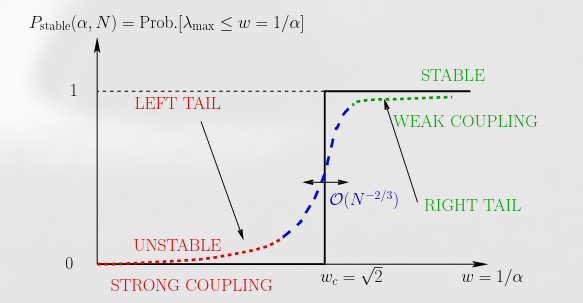
\includegraphics[width=0.5\linewidth]{./Assets/RegimeTW.png}
\end{figure}

In the thermodynamic equations describing water, the curve that represents the water’s energy as a function of temperature has a kink at 100 degrees Celsius, the point at which the liquid becomes steam. The water’s energy slowly increases up to this point, suddenly jumps to a new level and then slowly increases again along a different curve, in the form of steam. Crucially, where the energy curve has a kink, the “first derivative” of the curve has a peak.

Similarly, the physicists realized, the energy curves of certain strongly correlated systems have a kink at $\sqrt{2N}$. The associated peak for these systems is the Tracy-Widom distribution, which appears in the third derivative of the energy curve — that is, the rate of change of the rate of change of the energy’s rate of change. This makes the Tracy-Widom distribution a “third-order” phase transition.
